\documentclass[10pt,a4paper]{article}
\usepackage[T1]{fontenc}
\usepackage[utf8]{inputenc}
\usepackage{lmodern,microtype}
\usepackage[margin=0.83in]{geometry}
\usepackage{amsmath,amssymb,amsthm,mathtools,bm}
\usepackage{booktabs,array,tabularx}
\usepackage{xcolor,hyperref}
\usepackage{tikz}
\usetikzlibrary{arrows.meta,positioning}
\usepackage{enumitem,fancyhdr}
\hypersetup{colorlinks=true,linkcolor=blue!50!black,urlcolor=blue!55!black,citecolor=blue!45!black}
\definecolor{deep}{HTML}{183C54}
\definecolor{turq}{HTML}{117C80}
\definecolor{graytone}{HTML}{687783}
\setlength{\parindent}{0pt}
\setlength{\parskip}{4.2pt}
\setlist[itemize]{leftmargin=*,topsep=3pt,itemsep=2pt}
\setlist[enumerate]{leftmargin=*,topsep=3pt,itemsep=2pt}
\pagestyle{fancy}
\fancyhf{}
\fancyhead[L]{\footnotesize\textcolor{graytone}{REFLEX / TECHNICAL RESEARCH NOTE}}
\fancyhead[R]{\footnotesize\textcolor{graytone}{22 November 2026}}
\fancyfoot[C]{\footnotesize\textcolor{graytone}{\thepage}}
\renewcommand{\headrulewidth}{0.3pt}
\newtheorem{theorem}{Theorem}
\newtheorem{lemma}[theorem]{Lemma}
\newtheorem{proposition}[theorem]{Proposition}
\newtheorem{corollary}[theorem]{Corollary}
\theoremstyle{definition}\newtheorem{definition}[theorem]{Definition}
\newcommand{\F}{\mathbb F_2}
\newcommand{\wt}{\operatorname{wt}}
\newcommand{\im}{\operatorname{im}}
\newcommand{\dist}{\operatorname{dist}}
\begin{document}
\begin{center}
{\Large\bfseries\textcolor{deep}{Authority Graphs as Error-Correcting Evidence}}\\[4pt]
{\large\textcolor{turq}{An Identifiability and Corruption Frontier for Delegated Multi-Agent Audits}}\\[9pt]
{\normalsize\bfseries REFLEX-T / Working theoretical research draft}\\[3pt]
{\small Research direction developed for Mohammad Amanlou, University of Tehran}\\[3pt]
{\footnotesize\textcolor{graytone}{Pre-submission research note. Not peer reviewed; claims of historical novelty and publication readiness not established.}}
\end{center}
\noindent{\footnotesize\textbf{Code and reproducibility: }\url{https://github.com/MohammadAmanlou/REFLEX}}\par\vspace{4pt}
\vspace{-5pt}
\begin{abstract}
\noindent Delegated AI systems may contain multiple autonomous agents reporting evidence on behalf of the same principal. A central difficulty is that their reports can be distorted by shared reporting conventions or strategic preferences, while audit authority is restricted. We introduce a deliberately narrow \emph{authority-gated audit graph} model in which an unknown decision-relevant bit is encoded in pairwise audits, agents possess unrestricted but consistent latent binary offsets, and a limited number of edge reports may be corrupted. We characterize identifiability by a cycle-space obstruction, exact adversarial corruption tolerance by a coset distance, and the computational boundary between finding a cheapest noiseless witness and computing general robustness. We also give a constructive edge-disjoint-cycle certificate and exact finite-instance tests. The mathematical ingredients overlap classical signed-graph balance, group synchronization, and binary coding; the model and its proof obligations are a starting point for studying \emph{strategically implementable} audit rights, not a claimed new conference-level result. The central open research challenge is to endogenize the audit graph in a multi-principal game and prove that incentive-compatible delegation enforces the consistency assumptions needed for these certificates.
\end{abstract}
\vspace{-5pt}
\section{Motivation and literature boundary}
A multi-agent system may perform a delegated task under several local reports without a single globally trustworthy reporter. If one agent is replicated, a scheme based on the number of agreeing reports can become overconfident. If every report is treated as fully adversarial, however, no nontrivial statistical statement follows without independent verification or structural restrictions. We therefore ask: \emph{what part of a decision-relevant fact survives arbitrary, but structurally consistent, changes in agents' reporting conventions?}

The question sits near several well-developed literatures. Davoust and Rovatsos \cite{davoust2020} analyze incentive-compatible social contracts. Sourbut, Hammond and Wood \cite{sourbut2024} formalize cooperation and control in delegation games. Cacciamani, Castiglioni and Gatti \cite{cacciamani2024} give an optimal information-acquisition mechanism for multiple strategic agents, including equilibrium constraints. Das, Yu and Zhang \cite{das2026} directly optimize audit policies against adversarial agents and pessimistic equilibrium selection. Lerman and Shi \cite{lerman2022} use cycle consistency for adversarially corrupted group synchronization. The signed-graph frustration index and its relation to Max-Cut are classical \cite{aref2019}.

\textbf{Positioning.} We do not claim that cycle parity, syndrome decoding, shortest odd cycles, or the frustration index are inventions of REFLEX-T. Instead, we investigate whether these precise guarantees can become \emph{incentive-compatible institutional guarantees} under auditable delegation and multiple human principals. The present note develops and checks the restricted algebraic subproblem; it does not complete that extension.

\section{Authority-gated observations and adversarial conventions}
Let $G=(V,E)$ be a finite, undirected audit graph with no loops. Nodes represent delegated agent contexts whose reporting conventions may differ; an edge represents a pairwise comparison that an authorized institution can actually execute. Let $h\in\F$ be a binary \emph{decision-relevant} state, such as which of two candidate agreements passes a specified objective test. Let $s_v\in\F$ be an unrestricted hidden reporting convention for node $v$; these may be chosen strategically, but must remain the \emph{same on every incident edge within an audit episode}. Each edge has a \emph{known, verified} sensitivity bit $b_e\in\F$ indicating how its comparison responds to $h$.

The complete observed bit on an authorized edge $e=\{u,v\}$ is
\begin{equation}\label{eq:obs}
 y_e=s_u\oplus s_v\oplus(b_e h)\oplus\eta_e.
\end{equation}
Here $\eta_e$ denotes corruption, not an assumption of honest agent speech. With arbitrary per-edge $\eta_e$, no certificate is possible. We therefore make one of two explicit assumptions: (i) $\wt(\eta)\le t$ adversarial bit flips in an episode, or (ii) independent bit flips with known rates for repeated authorized episodes. The model requires the institution to verify the audit edge, the sensitivity $b_e$, and the consistency of a node's reported convention across incident edges. A cryptographic identity token alone would \emph{not} verify the underlying semantic facts or these economic assumptions.

Let $D\in\F^{|E|\times|V|}$ be the undirected vertex-edge incidence matrix over $\F$, with two ones per row. In vector form,
\begin{equation}\label{eq:matrix}
 y=Ds\oplus bh\oplus\eta.
\end{equation}
The model quantifies over \emph{all} $s\in\F^{|V|}$, including colluding node offsets. However it is not yet a fully specified principal-agent game: the consistency rule and corruption budget are exogenous institutional assumptions. Deriving them endogenously from payoffs is the core future contribution.

\begin{figure}[t]
\centering
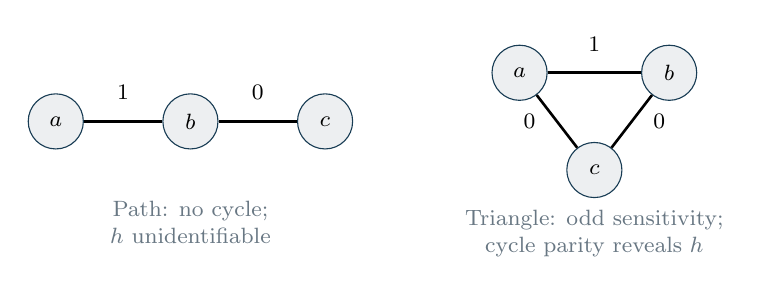
\begin{tikzpicture}[every node/.style={font=\footnotesize}, scale=.95]
\tikzstyle{vtx}=[circle,draw=deep,fill=deep!8,minimum size=7mm,inner sep=1pt]
\node[vtx] (a) at (0,0) {$a$}; \node[vtx] (b) at (1.8,0) {$b$}; \node[vtx] (c) at (3.6,0) {$c$};
\draw[line width=.95pt] (a)--node[above=4pt] {$1$}(b)--node[above=4pt] {$0$}(c);
\node at (1.8,-1.35) [align=center,text=graytone] {Path: no cycle;\\ $h$ unidentifiable};
\node[vtx] (d) at (6.2,.65) {$a$}; \node[vtx] (e) at (8.2,.65) {$b$}; \node[vtx] (f) at (7.2,-.65) {$c$};
\draw[line width=.95pt] (d)--node[above=4pt] {$1$}(e);
\draw[line width=.95pt] (e)--node[right=4pt] {$0$}(f);
\draw[line width=.95pt] (f)--node[left=4pt] {$0$}(d);
\node at (7.2,-1.5) [align=center,text=graytone] {Triangle: odd sensitivity;\\ cycle parity reveals $h$};
\end{tikzpicture}
\caption{Two graph topologies with the same three agents but different identifiability. A path admits an offset reparameterization that hides $h$; a parity-sensitive cycle cancels all node offsets.}
\end{figure}

\section{Exact identifiability frontier}
For $h\in\F$ define the set of uncorrupted feasible transcripts
\begin{equation}\label{eq:cosets}
 \mathcal C_h=\{Ds\oplus bh:s\in\F^{|V|}\}.
\end{equation}
A cycle is \emph{$b$-odd} when the XOR of its sensitivity bits is one.

\begin{theorem}[Exact identifiability]\label{thm:zero}
In model \eqref{eq:matrix} with $\eta=0$, the state $h$ is identifiable for every possible strategic offset $s$ if and only if
\[
 b\notin\im(D).
\]
Equivalently, $G$ contains a $b$-odd cycle.
\end{theorem}
\begin{proof}
Two hypotheses produce a common transcript precisely when $Ds_0=Ds_1\oplus b$, equivalent to $b=D(s_0\oplus s_1)$. Hence their transcript sets are disjoint exactly when $b\notin\im(D)$. If $b=Ds$, every cycle has zero XOR because each vertex appears twice. Conversely, pick a spanning forest, define vertex labels by XOR sums along tree paths, and note that the absence of any $b$-odd fundamental cycle implies $b_e=s_u\oplus s_v$ on each non-tree edge as well. Thus $b\in\im(D)$ exactly when all cycles are $b$-even.
\end{proof}

\textbf{Example.} For the path $a-b-c$ with $b=(1,0)$, the worlds $h=0,s=(0,0,0)$ and $h=1,s=(1,0,0)$ both produce $y=(0,0)$. Add a closing edge $c-a$ with $b=0$: every cycle XOR equals $h$ since each $s_v$ occurs twice. This is a \emph{topological obstruction}, but it is also a standard consequence of signed-graph balance and cycle-space algebra, not a new mathematical primitive.

\section{Adversarial corruption and a coding frontier}
Define the minimum coset separation (frustration distance)
\begin{equation}\label{eq:dist}
 d_*(G,b)=\min_{s\in\F^{|V|}}\wt(b\oplus Ds).
\end{equation}
Let $\mathcal B_t(\mathcal C_h)$ be the Hamming ball of radius $t$ around the set of all transcripts from hypothesis $h$.

\begin{theorem}[Exact Byzantine-edge tolerance]\label{thm:t}
The decision-relevant state $h$ can be determined uniquely from any authorized transcript for all node offsets and at most $t$ adversarially corrupted edges if and only if
\begin{equation}\label{eq:threshold}
 d_*(G,b)>2t.
\end{equation}
\end{theorem}
\begin{proof}
The minimum Hamming distance between $\mathcal C_0$ and $\mathcal C_1$ is exactly $d_*$: for any $s_0,s_1$, $\wt(Ds_0\oplus b\oplus Ds_1)=\wt(b\oplus D(s_0\oplus s_1))$. If $d_*>2t$, the two radius-$t$ balls do not intersect by the triangle inequality, so nearest-coset decoding uniquely identifies $h$. If $d_*\le2t$, choose two codewords at distance $d_*$ and construct an intermediate transcript differing from each on at most $t$ positions by splitting their differing coordinates. The same transcript is then compatible with both hypotheses, making uniform identification impossible.
\end{proof}

\begin{corollary}[Multi-bit extension]
Suppose $h\in\F^k$ and $y=Ds\oplus Ch\oplus\eta$, with known $C\in\F^{|E|\times k}$. The vector $h$ is identifiable in the noiseless model if and only if the image of $C$ in the quotient space $\F^{|E|}/\im(D)$ has rank $k$. With up to $t$ arbitrary edge flips, unique identification is possible if and only if
\[
 \min_{\Delta h\ne0}\min_{s}\wt(C\Delta h\oplus Ds)>2t.
\]
\end{corollary}
\begin{proof}
Two states $h$ and $h'$ have a common noiseless transcript iff $C(h-h')\in\im(D)$. This is excluded for nonzero differences exactly when the quotient map is injective, or has rank $k$. The error threshold follows by applying the Hamming-ball argument of Theorem~\ref{thm:t} to every pair of distinct messages.
\end{proof}

\section{Algorithms and limits of efficient certification}
\begin{theorem}[Cheapest uncorrupted witness]
When edge audit costs $c_e$ are strictly positive, a minimum-cost set of edge audits that certifies $h$ in the noiseless model can be chosen as a minimum-cost $b$-odd simple cycle. It can be found in polynomial time via a two-layer parity-expanded graph.
\end{theorem}
\begin{proof}
Any certifying edge subset must contain a $b$-odd cycle by Theorem~\ref{thm:zero}. Since all costs are positive, an optimal witness never needs extra edges outside one such cycle. Replace every vertex $v$ with $(v,0)$ and $(v,1)$; each original edge $\{u,v\}$ of sensitivity $b_e$ becomes a transition $(u,p)\leftrightarrow(v,p\oplus b_e)$ of cost $c_e$. For every root $v$, a shortest path from $(v,0)$ to $(v,1)$ projects to a $b$-odd closed walk. Any odd closed walk decomposes into cycles, at least one of which is $b$-odd and costs no more. Taking the best root thus recovers the globally cheapest odd cycle. Dijkstra from every root takes polynomial time, e.g., $O(|V|(|E|+|V|)\log |V|)$ with ordinary heaps.
\end{proof}

\begin{theorem}[Hardness of exact robust distance]
Computing $d_*(G,b)$ is NP-hard on general graphs.
\end{theorem}
\begin{proof}
Set $b_e=1$ for every edge. For a node labelling $s$, the quantity $\wt(b\oplus Ds)$ counts edges whose endpoints receive the same label, since $(1\oplus s_u\oplus s_v)=1$ exactly for equal endpoint bits. Thus $d_*(G,\mathbf1)=|E|-\operatorname{MaxCut}(G)$. A polynomial-time algorithm for $d_*$ would give a polynomial-time algorithm for Max-Cut.
\end{proof}

The hardness proof reduces to a familiar signed-graph frustration-index fact \cite{aref2019}; it must not be represented as a new complexity breakthrough.

\begin{proposition}[Constructive corruption certificate]
If the authorized graph has $2t+1$ \emph{edge-disjoint} $b$-odd cycles, a majority vote over their observed cycle parities recovers $h$ despite any $t$ corrupted edge reports, for every node-offset vector $s$.
\end{proposition}
\begin{proof}
XOR along each cycle eliminates $Ds$ and returns $h$ unless the cycle contains an odd number of corrupted edges. Since cycles are edge-disjoint, each corrupted edge can spoil at most one parity vote. At most $t$ of the $2t+1$ cycle votes are incorrect; a strict majority is correct.
\end{proof}

The packing rule is \emph{sufficient but not necessary}; it may be incomplete even when the optimal coset-distance decoder succeeds. A greedy algorithm that repeatedly finds and removes a cheapest $b$-odd cycle constructs a valid certificate whenever it reaches the required count, but need not discover one whenever one exists.

\section{A restricted incentive-compatible audit layer}
The preceding results quantify over arbitrary node offsets but assume that an edge-level audit reports the specified comparison, except for a bounded number of corruptions. An institution needs a reason to expect this condition. The following simple mechanism makes that issue explicit; it is not intended as a replacement for full Bayesian mechanism design.

For each selected edge $e$, suppose a separate reporting agent chooses either the prescribed edge comparison or its bit-flipped version. Assume that, holding every other report and decision fixed, the benefit of flipping is at most $g_e\ge0$ in \emph{every} possible state. The institution privately audits the edge against an external reference with probability $q_e$, detects a false edge report without error, and imposes enforceable penalty $F_e>0$. The expected cost of an audit opportunity is $c_eq_e$. A fixed incentive margin $\kappa>0$ is required. Node conventions are freely chosen but bindingly committed before edge comparison; this is a separate protocol assumption.

\begin{proposition}[One-cycle strict-incentive audit design]\label{prop:strategic}
Restrict mechanisms to a single parity-sensitive cycle, one independent agent per selected edge, mandatory participation, and independent audit coins. Suppose $F_e\ge g_e+\kappa$ on each usable edge. Setting
\begin{equation}\label{eq:incentives}
 q_e=\frac{g_e+\kappa}{F_e}
\end{equation}
ensures every selected reporter strictly prefers an unmodified edge report under all strategies of the others. Thus every Nash equilibrium in the reporting subgame yields the correct cycle parity. Within this mechanism class and this \emph{uniform incentive-margin certificate}, the minimum audit expenditure is the cost of a cheapest $b$-odd cycle with edge weights
\[
 w_e=c_e(g_e+\kappa)/F_e,
\]
found by the parity-lifted shortest-path algorithm.
\end{proposition}
\begin{proof}
Conditional on others' decisions, the benefit of flipping before enforcement is bounded by $g_e$, while a detected flip loses $F_e$ with probability $q_e$. With the stated $q_e$, the expected net advantage of a flip is at most $g_e-q_eF_e=-\kappa<0$. Therefore honest edge reporting is strictly dominant for each selected independent reporter; in every equilibrium each selected edge carries the prescribed comparison. The parity of an authorized $b$-odd cycle then cancels all (committed) node offsets and equals $h$. To certify this strict uniform margin using the assumed gain bound, each selected edge requires $q_eF_e\ge g_e+\kappa$; any larger $q_e$ costs more. By Theorem~\ref{thm:zero}, any successful single-cycle mechanism must select a $b$-odd cycle; minimizing the sum of resulting per-edge audit costs is exactly the shortest parity-odd cycle problem.
\end{proof}

\textbf{Scope and novelty caveat.} This proposition is a simple domination argument coupled with a graph algorithm. It does not cover correlated agents, coordinated multi-edge deviations by one agent, uncertain audit validity, weak penalties, endogenous participation, or several principals with conflicting utility. Its potential value is to state an explicit \emph{bridge} between strategic behavior and structural identifiability; it is not yet a novel general incentive-compatibility theorem.

\section{Stochastic error and abstention}
Assume edge flips on cycle $C$ are independent Bernoulli with rates $p_e<1/2$ in each fresh episode. Since XOR is a parity transform, the probability that the cycle-bit is incorrect is
\begin{equation}\label{eq:noise}
 q_C=\frac{1-\prod_{e\in C}(1-2p_e)}{2}.
\end{equation}
Across $N$ independent episodes the node offsets may vary arbitrarily; they cancel in each cycle. Majority voting on its cycle-bits and Hoeffding's inequality give
\begin{equation}
 \Pr(\widehat h\ne h)\le\exp\!\left(-\frac{N}{2}\left[\prod_{e\in C}(1-2p_e)\right]^2\right).
\end{equation}
This is a correctness bound under the stated noise and repeated-episode assumptions, not a guarantee for arbitrarily colluding edge corruptions. For higher-corruption environments, the decoder should \emph{abstain} when the nearest two cosets have equal Hamming distance, rather than invent a confident conclusion.

\section{Reproducible computational checks}
The accompanying standard-library Python implementation constructs the cosets exactly on small graphs; checks the least-cost odd cycle against exhaustive simple-cycle enumeration on 100 randomized graphs; and verifies the majority-packing certificate on all offsets and single-edge corruption patterns in a three-triangle instance. These are \emph{sanity checks}, not an empirical comparison with contemporary LLM systems or mechanism-design baselines.

\begin{table}[h]
\centering\small
\caption{Exact small-instance results obtained with the accompanying executable.}
\begin{tabular}{@{}lrrrr@{}}\toprule
Graph & $|V|$ & $|E|$ & $d_*$ & Guaranteed corrupted edges $t$ \\\midrule
Path, one sensitive edge & 3 & 2 & 0 & none \\
Triangle, one sensitive edge & 3 & 3 & 1 & 0 \\
$K_5$, all edges sensitive & 5 & 10 & 4 & 1 \\\bottomrule
\end{tabular}
\end{table}

For $K_5$, with ten independent edge flip probabilities $p_e=0.05$, the event ``at most one flip'' has probability $0.913862$ and is covered by the worst-case correction theorem. Exact enumeration of all $2^{10}$ noise patterns under a nearest-coset decoder that abstains on distance ties gives: correct $0.915652$, abstention $0.080788$, error $0.003559$. The two values of $h$ give symmetric results. A separate instance consisting of three edge-disjoint parity-sensitive triangles is proved correct by exhaustive enumeration of $2^9$ node conventions and all 10 error masks containing zero or one corrupt edge, for each $h$. These figures describe the toy audit model only.

\section{What would constitute a genuinely new conference paper?}
\textbf{The current mathematics is not enough for a top-tier novelty claim.} Three structural additions are needed before REFLEX-T could make a strong publication claim.

\textbf{A. Endogenous strategic consistency.} Instead of assuming one stable offset $s_v$ per node, define a multi-principal Bayesian or extensive-form game where agents can strategically submit distinct incident-edge reports. Specify enforceable deposits, bounded penalties, cross-check requests, limited audit budgets, and an outside option. Prove an equilibrium-robust mechanism theorem that makes the consistency premise of \eqref{eq:obs} valid under explicit incentive and participation constraints, or characterize when this is impossible. It is not sufficient to add payments without proving all relevant strategic deviations unprofitable. This must be compared theorem-by-theorem with optimal multi-agent information acquisition \cite{cacciamani2024} and optimal adversarial auditing \cite{das2026}.

\textbf{B. Authority design beyond signed-graph reconstruction.} Let an institution choose a permitted edge set $E'\subseteq E$ under stakeholder authorization and audit costs. Investigate the minimum-cost design that achieves $d_*(G',b')>2t$ \emph{and} implements the corresponding comparison protocol in all admissible equilibria. A combined hardness/tractability frontier would be more informative than either a standalone Max-Cut reduction or a shortest-cycle routine. Cost-sensitive adaptive audits, equilibrium selection, and multiple principals should not be assumed solved by classical coding arguments.

\textbf{C. Evidence-backed agent experiments.} Build tasks in which real LLM agent workflows can selectively duplicate, conceal, or distort evidence under known incentives. Compare with honest voting, independent auditing, optimal-audit game baselines and group synchronization methods. Report valid certificate rate, false certification, abstention, cost, and out-of-distribution stability, with uncertainty quantification and all failure cases. The present script does not establish these empirical properties.

\paragraph{Threat-model boundaries.} The hidden decision state must have an independently justified operational meaning; an edge sensitivity bit must be known from a verifiable protocol rather than defined to force the theorem; edge comparisons must be executable without unauthorized interference; adversarial offset consistency requires enforcement; no guarantee is claimed for arbitrarily changing node conventions per edge, unbounded corruption, biased noise with unknown parameters, or human preference manipulation. Without these safeguards the formal guarantees are not transferable to deployed agent systems.

\section{Research positioning for a potential supervisor}
The most suitable doctoral framing is not ``we invented cycle-based robustness.'' Rather: \emph{When can an institution induce autonomous agents with conflicting incentives to participate in a low-cost, auditable evidence graph whose topology certifies a principal-level decision, and when are such certificates information-theoretically impossible?} This retains the strongest thematic links to social contracts, incentives and multi-agent institutions in Rovatsos's research \cite{davoust2020}. The mathematically completed subproblem here gives a foundation and a falsifiable experimental protocol; the actual novel contribution would require solving one of the strategic-implementation questions above. No supervisor support, funded position, or conference acceptance is implied.

\section*{Research-integrity status and next reproducibility gates}
\begin{itemize}
\item \textbf{Done:} clear restricted model; proved identifiability, exact corruption threshold, and shortest witness; derived known hardness reduction and a sufficient packing rule; programmatically tested 100 random instances and exact small-graph outcomes.
\item \textbf{Not done:} proof of publication priority over signed-graph synchronization and audit mechanism design; full strategic equilibrium model; new efficient mechanism under endogenous authority; real or simulated LLM-agent benchmark, comparisons, ablations, statistical significance; an actual submitted manuscript.
\item \textbf{Required before submission:} independent proof verification, exhaustive related-work search with expert feedback, baseline code reproduction, methodological and statistical review, appropriate conference formatting and anonymity requirements, and authorship/content review by Mohammad.
\end{itemize}

\begin{thebibliography}{9}\small
\bibitem{davoust2020} A. Davoust and M. Rovatsos. Social Contracts for Non-Cooperative Games. \emph{AIES}, 2020. \url{https://homepages.inf.ed.ac.uk/mrovatso/papers/davoust-rovatsos-aies2020.pdf}.
\bibitem{sourbut2024} O. Sourbut, L. Hammond and H. Wood. Cooperation and Control in Delegation Games. \emph{IJCAI}, 2024. \url{https://www.ijcai.org/proceedings/2024/26}.
\bibitem{cacciamani2024} F. Cacciamani, M. Castiglioni and N. Gatti. Online Information Acquisition: Hiring Multiple Agents. \emph{ICLR}, 2024. \url{https://mlanthology.org/iclr/2024/cacciamani2024iclr-online/}.
\bibitem{das2026} S. Das, F.-Y. Yu and Y. Zhang. Optimally Auditing Adversarial Agents. \emph{AAAI}, 2026. \url{https://ojs.aaai.org/index.php/AAAI/article/download/38722/42684}.
\bibitem{lerman2022} G. Lerman and Y. Shi. Robust Group Synchronization via Cycle-Edge Message Passing. \emph{Foundations of Computational Mathematics}, 22:1665--1741, 2022. \url{https://link.springer.com/article/10.1007/s10208-021-09532-w}.
\bibitem{aref2019} \emph{A Modeling and Computational Study of the Frustration Index in Signed Networks}. \emph{Networks}, 2019/2020. \url{https://doi.org/10.1002/net.21907}.
\bibitem{tewolde2024} E. Tewolde et al. Game Transformations That Preserve Nash Equilibria or Best-Response Sets. \emph{IJCAI}, 2024. \url{https://ijcai.org/proceedings/2024/331}.
\bibitem{erdogan2026} M. Erdogan et al. Who Should Know What? Empirical Information Design for Multi-Agent LLM Economies. arXiv:2611.07667, 2026. \url{https://arxiv.org/abs/2611.07667}.
\end{thebibliography}
\end{document}
